% Options for packages loaded elsewhere
\PassOptionsToPackage{unicode}{hyperref}
\PassOptionsToPackage{hyphens}{url}
%
\documentclass[
]{article}
\usepackage{amsmath,amssymb}
\usepackage{lmodern}
\usepackage{ifxetex,ifluatex}
\ifnum 0\ifxetex 1\fi\ifluatex 1\fi=0 % if pdftex
  \usepackage[T1]{fontenc}
  \usepackage[utf8]{inputenc}
  \usepackage{textcomp} % provide euro and other symbols
\else % if luatex or xetex
  \usepackage{unicode-math}
  \defaultfontfeatures{Scale=MatchLowercase}
  \defaultfontfeatures[\rmfamily]{Ligatures=TeX,Scale=1}
\fi
% Use upquote if available, for straight quotes in verbatim environments
\IfFileExists{upquote.sty}{\usepackage{upquote}}{}
\IfFileExists{microtype.sty}{% use microtype if available
  \usepackage[]{microtype}
  \UseMicrotypeSet[protrusion]{basicmath} % disable protrusion for tt fonts
}{}
\makeatletter
\@ifundefined{KOMAClassName}{% if non-KOMA class
  \IfFileExists{parskip.sty}{%
    \usepackage{parskip}
  }{% else
    \setlength{\parindent}{0pt}
    \setlength{\parskip}{6pt plus 2pt minus 1pt}}
}{% if KOMA class
  \KOMAoptions{parskip=half}}
\makeatother
\usepackage{xcolor}
\IfFileExists{xurl.sty}{\usepackage{xurl}}{} % add URL line breaks if available
\IfFileExists{bookmark.sty}{\usepackage{bookmark}}{\usepackage{hyperref}}
\hypersetup{
  pdftitle={西南大学 2022: STATS 201 Assignment 2},
  pdfauthor={Your Name and ID Number here},
  hidelinks,
  pdfcreator={LaTeX via pandoc}}
\urlstyle{same} % disable monospaced font for URLs
\usepackage[margin=1in]{geometry}
\usepackage{color}
\usepackage{fancyvrb}
\newcommand{\VerbBar}{|}
\newcommand{\VERB}{\Verb[commandchars=\\\{\}]}
\DefineVerbatimEnvironment{Highlighting}{Verbatim}{commandchars=\\\{\}}
% Add ',fontsize=\small' for more characters per line
\usepackage{framed}
\definecolor{shadecolor}{RGB}{248,248,248}
\newenvironment{Shaded}{\begin{snugshade}}{\end{snugshade}}
\newcommand{\AlertTok}[1]{\textcolor[rgb]{0.94,0.16,0.16}{#1}}
\newcommand{\AnnotationTok}[1]{\textcolor[rgb]{0.56,0.35,0.01}{\textbf{\textit{#1}}}}
\newcommand{\AttributeTok}[1]{\textcolor[rgb]{0.77,0.63,0.00}{#1}}
\newcommand{\BaseNTok}[1]{\textcolor[rgb]{0.00,0.00,0.81}{#1}}
\newcommand{\BuiltInTok}[1]{#1}
\newcommand{\CharTok}[1]{\textcolor[rgb]{0.31,0.60,0.02}{#1}}
\newcommand{\CommentTok}[1]{\textcolor[rgb]{0.56,0.35,0.01}{\textit{#1}}}
\newcommand{\CommentVarTok}[1]{\textcolor[rgb]{0.56,0.35,0.01}{\textbf{\textit{#1}}}}
\newcommand{\ConstantTok}[1]{\textcolor[rgb]{0.00,0.00,0.00}{#1}}
\newcommand{\ControlFlowTok}[1]{\textcolor[rgb]{0.13,0.29,0.53}{\textbf{#1}}}
\newcommand{\DataTypeTok}[1]{\textcolor[rgb]{0.13,0.29,0.53}{#1}}
\newcommand{\DecValTok}[1]{\textcolor[rgb]{0.00,0.00,0.81}{#1}}
\newcommand{\DocumentationTok}[1]{\textcolor[rgb]{0.56,0.35,0.01}{\textbf{\textit{#1}}}}
\newcommand{\ErrorTok}[1]{\textcolor[rgb]{0.64,0.00,0.00}{\textbf{#1}}}
\newcommand{\ExtensionTok}[1]{#1}
\newcommand{\FloatTok}[1]{\textcolor[rgb]{0.00,0.00,0.81}{#1}}
\newcommand{\FunctionTok}[1]{\textcolor[rgb]{0.00,0.00,0.00}{#1}}
\newcommand{\ImportTok}[1]{#1}
\newcommand{\InformationTok}[1]{\textcolor[rgb]{0.56,0.35,0.01}{\textbf{\textit{#1}}}}
\newcommand{\KeywordTok}[1]{\textcolor[rgb]{0.13,0.29,0.53}{\textbf{#1}}}
\newcommand{\NormalTok}[1]{#1}
\newcommand{\OperatorTok}[1]{\textcolor[rgb]{0.81,0.36,0.00}{\textbf{#1}}}
\newcommand{\OtherTok}[1]{\textcolor[rgb]{0.56,0.35,0.01}{#1}}
\newcommand{\PreprocessorTok}[1]{\textcolor[rgb]{0.56,0.35,0.01}{\textit{#1}}}
\newcommand{\RegionMarkerTok}[1]{#1}
\newcommand{\SpecialCharTok}[1]{\textcolor[rgb]{0.00,0.00,0.00}{#1}}
\newcommand{\SpecialStringTok}[1]{\textcolor[rgb]{0.31,0.60,0.02}{#1}}
\newcommand{\StringTok}[1]{\textcolor[rgb]{0.31,0.60,0.02}{#1}}
\newcommand{\VariableTok}[1]{\textcolor[rgb]{0.00,0.00,0.00}{#1}}
\newcommand{\VerbatimStringTok}[1]{\textcolor[rgb]{0.31,0.60,0.02}{#1}}
\newcommand{\WarningTok}[1]{\textcolor[rgb]{0.56,0.35,0.01}{\textbf{\textit{#1}}}}
\usepackage{graphicx}
\makeatletter
\def\maxwidth{\ifdim\Gin@nat@width>\linewidth\linewidth\else\Gin@nat@width\fi}
\def\maxheight{\ifdim\Gin@nat@height>\textheight\textheight\else\Gin@nat@height\fi}
\makeatother
% Scale images if necessary, so that they will not overflow the page
% margins by default, and it is still possible to overwrite the defaults
% using explicit options in \includegraphics[width, height, ...]{}
\setkeys{Gin}{width=\maxwidth,height=\maxheight,keepaspectratio}
% Set default figure placement to htbp
\makeatletter
\def\fps@figure{htbp}
\makeatother
\setlength{\emergencystretch}{3em} % prevent overfull lines
\providecommand{\tightlist}{%
  \setlength{\itemsep}{0pt}\setlength{\parskip}{0pt}}
\setcounter{secnumdepth}{-\maxdimen} % remove section numbering
\ifluatex
  \usepackage{selnolig}  % disable illegal ligatures
\fi

\title{西南大学 2022: STATS 201 Assignment 2}
\author{Your Name and ID Number here}
\date{Due date to be advised}

\begin{document}
\maketitle

\hypertarget{enter-your-name-here}{%
\subsection{Enter your name here}\label{enter-your-name-here}}

\begin{Shaded}
\begin{Highlighting}[]
\CommentTok{\# Replace "Model Student" with your name in quotes, }
\CommentTok{\# E.g., myname="Ruoxi Xu"}
\NormalTok{myname}\OtherTok{=}\StringTok{"runze liao"}
\end{Highlighting}
\end{Shaded}

\hypertarget{question-1}{%
\section{Question 1}\label{question-1}}

\hypertarget{background}{%
\subsection{Background}\label{background}}

A manufacturer of autonomous vehicles wanted to predict the stopping
distance as a function of vehicle speed (km/h).

Stopping distance (m) was measured as the distance traveled after
emergency braking was activated. You may assume that the observations
are independent.

The code below automatically generates the data for a randomly chosen
student. The data are in the dataframe \textbf{Stop.df}. Variable
\textbf{Speed} is the explanatory variable, and \textbf{Dist} is the
response variable.

\hypertarget{questions-of-interest}{%
\subsection{Questions of interest}\label{questions-of-interest}}

Make inference about the stopping distance for a given speed. In
particular,

\begin{itemize}
\tightlist
\item
  What is the effect of a doubling in speed?
\item
  Estimate the typical stopping distance for emergency braking at speeds
  of 50 km/h and 100 km/h.
\item
  The manufacturer desires that the vehicle stops in less than 12 m at
  50 km/h, at least 999 times out of 1000. Has this been achieved?
  {[}Hint, calculate the 0.998 level prediction interval.{]}
\end{itemize}

\begin{verbatim}
## Warning: package 's20x' was built under R version 4.0.5
\end{verbatim}

\hypertarget{plot-data}{%
\subsection{Plot data}\label{plot-data}}

\begin{Shaded}
\begin{Highlighting}[]
\CommentTok{\# Add R code below to draw appropriate scatter plot(s)}
\FunctionTok{plot}\NormalTok{(Dist}\SpecialCharTok{\textasciitilde{}}\NormalTok{Speed, }\AttributeTok{data =}\NormalTok{ Stop.df)}
\end{Highlighting}
\end{Shaded}

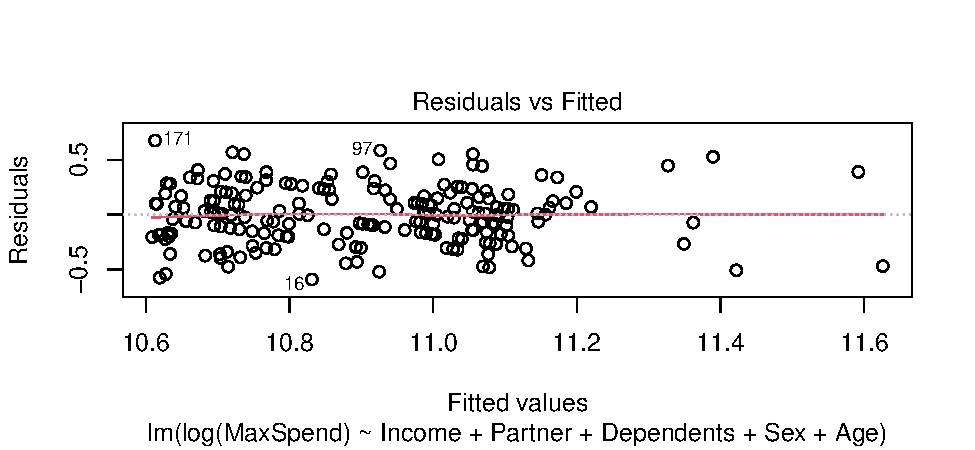
\includegraphics{STATS201_2022_SWU_A2_files/figure-latex/unnamed-chunk-4-1.pdf}

\begin{Shaded}
\begin{Highlighting}[]
\FunctionTok{plot}\NormalTok{(}\FunctionTok{log}\NormalTok{(Dist)}\SpecialCharTok{\textasciitilde{}}\NormalTok{Speed, }\AttributeTok{data =}\NormalTok{ Stop.df)}
\end{Highlighting}
\end{Shaded}

\includegraphics{STATS201_2022_SWU_A2_files/figure-latex/unnamed-chunk-5-1.pdf}

\begin{Shaded}
\begin{Highlighting}[]
\FunctionTok{plot}\NormalTok{(}\FunctionTok{log}\NormalTok{(Dist)}\SpecialCharTok{\textasciitilde{}}\FunctionTok{log}\NormalTok{(Speed), }\AttributeTok{data =}\NormalTok{ Stop.df)}
\end{Highlighting}
\end{Shaded}

\includegraphics{STATS201_2022_SWU_A2_files/figure-latex/unnamed-chunk-5-2.pdf}

\begin{Shaded}
\begin{Highlighting}[]
\FunctionTok{trendscatter}\NormalTok{(}\FunctionTok{log}\NormalTok{(Dist)}\SpecialCharTok{\textasciitilde{}}\FunctionTok{log}\NormalTok{(Speed),}\AttributeTok{data =}\NormalTok{ Stop.df)}
\end{Highlighting}
\end{Shaded}

\includegraphics{STATS201_2022_SWU_A2_files/figure-latex/unnamed-chunk-5-3.pdf}

In this graph, we can see a apparent looks reasonably linear on the log
scale and after we fit the log(Dist), it seems that it has a Power law
relation. So we will fit the model with log(Dist) and log(Speed)

\hypertarget{fit-a-power-law-model-and-do-assumption-checks}{%
\subsection{Fit a power-law model and do assumption
checks}\label{fit-a-power-law-model-and-do-assumption-checks}}

\begin{Shaded}
\begin{Highlighting}[]
\NormalTok{Stop.lm }\OtherTok{=} \FunctionTok{lm}\NormalTok{(}\FunctionTok{log}\NormalTok{(Dist)}\SpecialCharTok{\textasciitilde{}}\FunctionTok{log}\NormalTok{(Speed), }\AttributeTok{data =}\NormalTok{ Stop.df)}
\FunctionTok{plot}\NormalTok{(Stop.lm, }\AttributeTok{which =} \DecValTok{1}\NormalTok{)}
\end{Highlighting}
\end{Shaded}

\includegraphics{STATS201_2022_SWU_A2_files/figure-latex/unnamed-chunk-6-1.pdf}

\begin{Shaded}
\begin{Highlighting}[]
\FunctionTok{normcheck}\NormalTok{(Stop.lm)}
\end{Highlighting}
\end{Shaded}

\includegraphics{STATS201_2022_SWU_A2_files/figure-latex/unnamed-chunk-6-2.pdf}

\begin{Shaded}
\begin{Highlighting}[]
\FunctionTok{cooks20x}\NormalTok{(Stop.lm)}
\end{Highlighting}
\end{Shaded}

\includegraphics{STATS201_2022_SWU_A2_files/figure-latex/unnamed-chunk-6-3.pdf}
The EOV check is good, the residuals satisfy the normal distributions.
The point 3 seems strange, however, we will keep it as it does not
\textgreater{} 0.4.

\begin{Shaded}
\begin{Highlighting}[]
\FunctionTok{summary}\NormalTok{(Stop.lm)}
\end{Highlighting}
\end{Shaded}

\begin{verbatim}
## 
## Call:
## lm(formula = log(Dist) ~ log(Speed), data = Stop.df)
## 
## Residuals:
##       Min        1Q    Median        3Q       Max 
## -0.033919 -0.011019 -0.002776  0.014365  0.033273 
## 
## Coefficients:
##              Estimate Std. Error t value Pr(>|t|)    
## (Intercept) -5.467523   0.031587  -173.1   <2e-16 ***
## log(Speed)   2.000024   0.007064   283.1   <2e-16 ***
## ---
## Signif. codes:  0 '***' 0.001 '**' 0.01 '*' 0.05 '.' 0.1 ' ' 1
## 
## Residual standard error: 0.01859 on 26 degrees of freedom
## Multiple R-squared:  0.9997, Adjusted R-squared:  0.9997 
## F-statistic: 8.016e+04 on 1 and 26 DF,  p-value: < 2.2e-16
\end{verbatim}

\begin{Shaded}
\begin{Highlighting}[]
\FunctionTok{exp}\NormalTok{(}\FunctionTok{confint}\NormalTok{(Stop.lm))}
\end{Highlighting}
\end{Shaded}

\begin{verbatim}
##                   2.5 %      97.5 %
## (Intercept) 0.003956278 0.004504881
## log(Speed)  7.282719779 7.497311256
\end{verbatim}

The p-value of intercept and log(Speed) are all \textless{} 0.05, we
have strong evidence to believe the assumption.

The estimate of intercept is from 0.0040 to 0.0045 and the estimate of
Speed is from 7.28 to 7.50.

\hypertarget{inference-i.e-answer-questions-of-interest}{%
\subsection{Inference, i.e, answer questions of
interest}\label{inference-i.e-answer-questions-of-interest}}

\begin{Shaded}
\begin{Highlighting}[]
\CommentTok{\# Add R code below}
\NormalTok{pred.df }\OtherTok{=} \FunctionTok{data.frame}\NormalTok{(}\AttributeTok{Speed =} \FunctionTok{c}\NormalTok{(}\DecValTok{50}\NormalTok{,}\DecValTok{100}\NormalTok{))}
\FunctionTok{exp}\NormalTok{(}\FunctionTok{predict}\NormalTok{(Stop.lm,pred.df,}\AttributeTok{level =} \FloatTok{0.998}\NormalTok{, }\AttributeTok{interval =} \StringTok{"confidence"}\NormalTok{))}
\end{Highlighting}
\end{Shaded}

\begin{verbatim}
##        fit      lwr      upr
## 1 10.55520 10.37032 10.74338
## 2 42.22152 41.68918 42.76066
\end{verbatim}

If the Speed = 50, the Distance will be the 10.37 to 10.74, while when
the Speed = 100, then the distance will be 41.69 to 42.76.

\hypertarget{method-and-assumption-checks}{%
\subsection{Method and Assumption
Checks}\label{method-and-assumption-checks}}

By plotting the original data, we cannot find a linear regression, and
we use the Eov check and Normchenck, however, it does not satisfy by
fitting the simple linear regression. After logging the variables, the
scatter plots showed the desired linear relationship between Speed and
Distance, so we fitted a power law model explaining log Speed and log
Distance. The trendscatter using the power law model seems a straight
line. The underlying model assumptions appear valid, however, we have a
strange obseravtion point 3, however, it does not \textgreater{} 0.4, so
we will keep it. Our final model is:\\
\[log(Dist)_i = \beta_0 + \beta_1 * log(SpeWed)_i + \epsilon_i \] where
\(\epsilon_i\)\textasciitilde{}\(N(0,\sigma^2)\)

Our model explained 99.97\% of the vairability in the Speed \& Distance
model.

\hypertarget{executive-summary}{%
\subsection{Executive Summary}\label{executive-summary}}

We want to find the relationship between the Speed and the Distance, and
we also are interested in estimate the Speed.

The model was that the Distance would follow a power law relationship
with the car's Speed.\\
More specifically, the Distance will increase with the square of the
Speed.

The Distance will follow a power law modelwith respect to the Speed.

\begin{itemize}
\item
  What is the effect of a doubling in speed?\\
  As the power law parameter is 2, the Distance will increase with the
  square of the Speed, so the stop distance will be 4 times than before.
\item
  Estimate the typical stopping distance for emergency braking at speeds
  of 50 km/h and 100 km/h. We can see that If the Speed = 50, stopping
  distance for emergency braking be the 10.37 to 10.74, while when the
  Speed = 100, then stopping distance for emergency braking will be
  41.69 to 42.76.
\item
  The manufacturer desires that the vehicle stops in less than 12 m at
  50 km/h, at least 999 times out of 1000. Has this been achieved?
  {[}Hint, calculate the 0.998 level prediction interval.{]}\\
  If the Speed = 50, the Distance will be the 10.37 to 10.74, while when
  the Speed = 100, then the distance will be 41.69 to 42.76.
\end{itemize}

\newpage

\hypertarget{question-2}{%
\section{Question 2}\label{question-2}}

\hypertarget{background-and-questions-of-interest}{%
\subsection{Background and questions of
interest}\label{background-and-questions-of-interest}}

In New Zealand, the police are usually tolerant of speeding up to 10
km/h over the posted speed limit. However this tolerance is reduced to 5
km/h during public holidays.

We investigated the effect of the posted speed limit on the actual speed
of vehicles, and also the effect of the reduced police tolerance for
speeding that applies on holidays. Also, we wished to see if the effect
of the reduced tolerance during holidays depended on the posted speed
limit.

A total of 445 independent observations were made for posted speed
limits between 50 and 100 km/h. All measurements were made during
periods of unrestricted traffic flow on straight stretches of road.

\hypertarget{read-in-and-inspect-the-data}{%
\subsection{Read in and inspect the
data:}\label{read-in-and-inspect-the-data}}

\begin{Shaded}
\begin{Highlighting}[]
\NormalTok{Speed.df}\OtherTok{=}\FunctionTok{read.table}\NormalTok{(}\StringTok{"Speed.txt"}\NormalTok{, }\AttributeTok{header=}\NormalTok{T)}
\FunctionTok{plot}\NormalTok{(Speed}\SpecialCharTok{\textasciitilde{}}\NormalTok{Posted,}\AttributeTok{main=}\StringTok{"Actual Speed by Speed Limit and Holiday"}\NormalTok{, }\AttributeTok{col=}\FunctionTok{ifelse}\NormalTok{(Holiday}\SpecialCharTok{==}\StringTok{"N"}\NormalTok{,}\StringTok{"red"}\NormalTok{,}\StringTok{"blue"}\NormalTok{),}\AttributeTok{pch=}\FunctionTok{ifelse}\NormalTok{(Holiday}\SpecialCharTok{==}\StringTok{"N"}\NormalTok{,}\DecValTok{1}\NormalTok{,}\DecValTok{2}\NormalTok{),}\AttributeTok{data=}\NormalTok{Speed.df)}
\FunctionTok{legend}\NormalTok{(}\DecValTok{50}\NormalTok{,}\DecValTok{110}\NormalTok{,}\AttributeTok{pch=}\FunctionTok{c}\NormalTok{(}\DecValTok{1}\NormalTok{,}\DecValTok{2}\NormalTok{),}\AttributeTok{col=}\FunctionTok{c}\NormalTok{(}\StringTok{"red"}\NormalTok{,}\StringTok{"blue"}\NormalTok{),}\AttributeTok{legend=}\FunctionTok{c}\NormalTok{(}\StringTok{"Holiday"}\NormalTok{,}\StringTok{"Non{-}holiday"}\NormalTok{))}
\end{Highlighting}
\end{Shaded}

\includegraphics{STATS201_2022_SWU_A2_files/figure-latex/unnamed-chunk-9-1.pdf}

\hypertarget{comment-on-plot}{%
\subsection{Comment on plot}\label{comment-on-plot}}

The number of holiday cars is less than the Non-holidays. And we can see
that the average speed in their own posted area, the Holiday's Speed is
larger than the Non-holiday. The fact that appears this problem maybe in
holiday, the traffic management is easy.

\hypertarget{fit-model-and-check-assumptions}{%
\subsection{Fit model and check
assumptions}\label{fit-model-and-check-assumptions}}

\begin{Shaded}
\begin{Highlighting}[]
\CommentTok{\# Add R code below}
\FunctionTok{library}\NormalTok{(s20x)}
\NormalTok{Speed.fit }\OtherTok{=} \FunctionTok{lm}\NormalTok{(Speed}\SpecialCharTok{\textasciitilde{}}\NormalTok{Posted}\SpecialCharTok{*}\NormalTok{Holiday, }\AttributeTok{data =}\NormalTok{ Speed.df)}
\FunctionTok{plot}\NormalTok{(Speed.fit, }\AttributeTok{which =} \DecValTok{1}\NormalTok{)}
\end{Highlighting}
\end{Shaded}

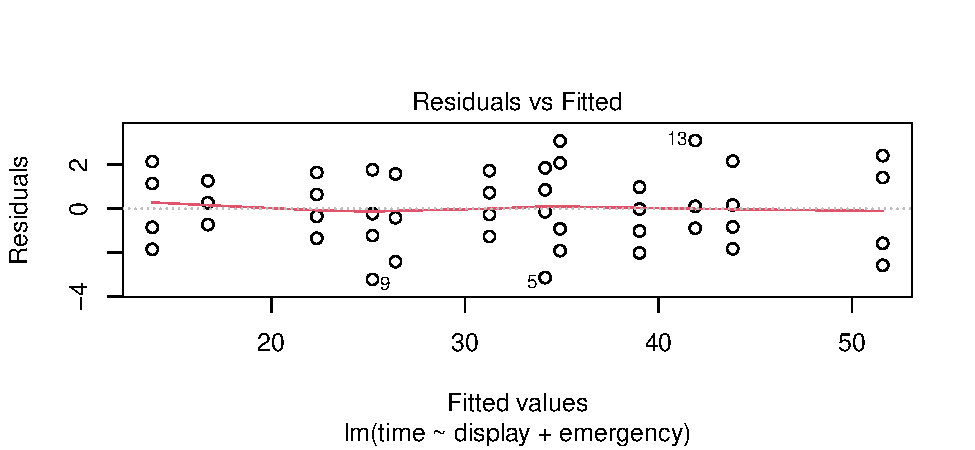
\includegraphics{STATS201_2022_SWU_A2_files/figure-latex/unnamed-chunk-10-1.pdf}

\begin{Shaded}
\begin{Highlighting}[]
\FunctionTok{normcheck}\NormalTok{(Speed.fit)}
\end{Highlighting}
\end{Shaded}

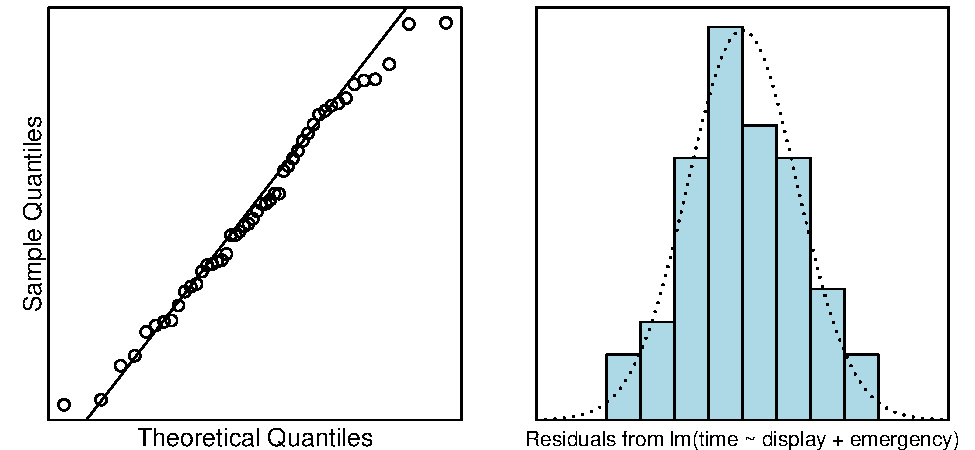
\includegraphics{STATS201_2022_SWU_A2_files/figure-latex/unnamed-chunk-10-2.pdf}

\begin{Shaded}
\begin{Highlighting}[]
\FunctionTok{cooks20x}\NormalTok{(Speed.fit)}
\end{Highlighting}
\end{Shaded}

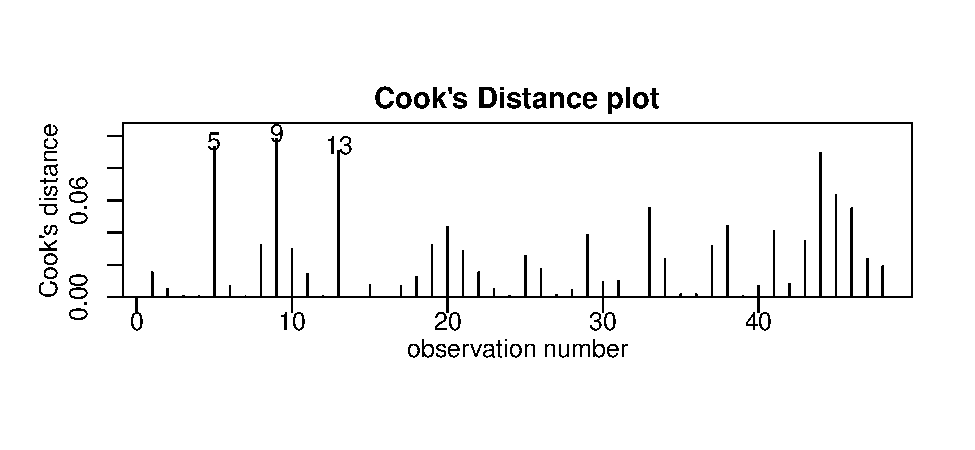
\includegraphics{STATS201_2022_SWU_A2_files/figure-latex/unnamed-chunk-10-3.pdf}

\begin{Shaded}
\begin{Highlighting}[]
\FunctionTok{summary}\NormalTok{(Speed.fit)}
\end{Highlighting}
\end{Shaded}

\begin{verbatim}
## 
## Call:
## lm(formula = Speed ~ Posted * Holiday, data = Speed.df)
## 
## Residuals:
##     Min      1Q  Median      3Q     Max 
## -8.5510 -1.9235  0.0614  1.8614  9.0490 
## 
## Coefficients:
##                  Estimate Std. Error t value Pr(>|t|)    
## (Intercept)      5.173458   1.061487   4.874 1.53e-06 ***
## Posted           0.998491   0.014727  67.801  < 2e-16 ***
## HolidayY        -5.247256   1.179569  -4.448 1.10e-05 ***
## Posted:HolidayY  0.005757   0.016346   0.352    0.725    
## ---
## Signif. codes:  0 '***' 0.001 '**' 0.01 '*' 0.05 '.' 0.1 ' ' 1
## 
## Residual standard error: 2.856 on 441 degrees of freedom
## Multiple R-squared:  0.9825, Adjusted R-squared:  0.9824 
## F-statistic:  8271 on 3 and 441 DF,  p-value: < 2.2e-16
\end{verbatim}

The residuals plot is good, the normcheck is good which indicates the
residuals are normally distributed. The all observations seem no strong
influence point.\\
However, through the summary we can see that the p-value of
Posted:HolidayY(0.725) is larger than 0.05 so much, so we wonder if we
can remove the interaction between the Posted and Holiday.

\hypertarget{reproduce-plot-with-fitted-lines-superimposed.}{%
\subsection{Reproduce plot with fitted lines
superimposed.}\label{reproduce-plot-with-fitted-lines-superimposed.}}

\begin{Shaded}
\begin{Highlighting}[]
\CommentTok{\# Add R code below}
\FunctionTok{trendscatter}\NormalTok{(Speed}\SpecialCharTok{\textasciitilde{}}\NormalTok{Posted, }\AttributeTok{data =}\NormalTok{ Speed.df)}
\end{Highlighting}
\end{Shaded}

\includegraphics{STATS201_2022_SWU_A2_files/figure-latex/unnamed-chunk-11-1.pdf}
The line between the holiday and Non-holiday is parallel, So we fitted
the model without interaction.

\begin{Shaded}
\begin{Highlighting}[]
\NormalTok{Speed.fit2 }\OtherTok{=} \FunctionTok{lm}\NormalTok{(}\AttributeTok{formula =}\NormalTok{ Speed }\SpecialCharTok{\textasciitilde{}}\NormalTok{ Posted }\SpecialCharTok{+}\NormalTok{ Holiday, }\AttributeTok{data =}\NormalTok{ Speed.df)}
\end{Highlighting}
\end{Shaded}

Then we plot some graphs to see if it satisfy all assumptions.

\begin{Shaded}
\begin{Highlighting}[]
\FunctionTok{plot}\NormalTok{(Speed.fit2, }\AttributeTok{which =} \DecValTok{1}\NormalTok{)}
\end{Highlighting}
\end{Shaded}

\includegraphics{STATS201_2022_SWU_A2_files/figure-latex/unnamed-chunk-13-1.pdf}

\begin{Shaded}
\begin{Highlighting}[]
\FunctionTok{normcheck}\NormalTok{(Speed.fit2)}
\end{Highlighting}
\end{Shaded}

\includegraphics{STATS201_2022_SWU_A2_files/figure-latex/unnamed-chunk-13-2.pdf}

\begin{Shaded}
\begin{Highlighting}[]
\FunctionTok{cooks20x}\NormalTok{(Speed.fit2)}
\end{Highlighting}
\end{Shaded}

\includegraphics{STATS201_2022_SWU_A2_files/figure-latex/unnamed-chunk-13-3.pdf}
From the graphs we could see that the Residuals is good, the
distribution of residuals is like Normal, the cooks distance is good, no
strong influence point. It satisfied all assumption.

\begin{Shaded}
\begin{Highlighting}[]
\FunctionTok{summary}\NormalTok{(Speed.fit2)}
\end{Highlighting}
\end{Shaded}

\begin{verbatim}
## 
## Call:
## lm(formula = Speed ~ Posted + Holiday, data = Speed.df)
## 
## Residuals:
##     Min      1Q  Median      3Q     Max 
## -8.5178 -1.9229  0.0589  1.8905  9.0822 
## 
## Coefficients:
##              Estimate Std. Error t value Pr(>|t|)    
## (Intercept)  4.851280   0.537983   9.018   <2e-16 ***
## Posted       1.003164   0.006383 157.153   <2e-16 ***
## HolidayY    -4.849907   0.344058 -14.096   <2e-16 ***
## ---
## Signif. codes:  0 '***' 0.001 '**' 0.01 '*' 0.05 '.' 0.1 ' ' 1
## 
## Residual standard error: 2.853 on 442 degrees of freedom
## Multiple R-squared:  0.9825, Adjusted R-squared:  0.9825 
## F-statistic: 1.243e+04 on 2 and 442 DF,  p-value: < 2.2e-16
\end{verbatim}

\begin{Shaded}
\begin{Highlighting}[]
\FunctionTok{confint}\NormalTok{(Speed.fit2)}
\end{Highlighting}
\end{Shaded}

\begin{verbatim}
##                  2.5 %    97.5 %
## (Intercept)  3.7939585  5.908602
## Posted       0.9906186  1.015709
## HolidayY    -5.5261009 -4.173713
\end{verbatim}

\begin{Shaded}
\begin{Highlighting}[]
\NormalTok{pred.df1 }\OtherTok{=} \FunctionTok{data.frame}\NormalTok{(}\AttributeTok{Posted =} \FunctionTok{c}\NormalTok{(}\DecValTok{50}\NormalTok{,}\DecValTok{60}\NormalTok{,}\DecValTok{70}\NormalTok{,}\DecValTok{80}\NormalTok{,}\DecValTok{90}\NormalTok{,}\DecValTok{100}\NormalTok{),}\AttributeTok{Holiday =} \StringTok{"Y"}\NormalTok{)}
\NormalTok{pred.df2 }\OtherTok{=} \FunctionTok{data.frame}\NormalTok{(}\AttributeTok{Posted =} \FunctionTok{c}\NormalTok{(}\DecValTok{50}\NormalTok{,}\DecValTok{60}\NormalTok{,}\DecValTok{70}\NormalTok{,}\DecValTok{80}\NormalTok{,}\DecValTok{90}\NormalTok{,}\DecValTok{100}\NormalTok{),}\AttributeTok{Holiday =} \StringTok{"N"}\NormalTok{)}
\FunctionTok{predict}\NormalTok{(Speed.fit2,pred.df1,}\AttributeTok{interval =} \StringTok{"confidence"}\NormalTok{)}
\end{Highlighting}
\end{Shaded}

\begin{verbatim}
##         fit      lwr       upr
## 1  50.15957 49.77704  50.54211
## 2  60.19121 59.87321  60.50922
## 3  70.22285 69.92723  70.51848
## 4  80.25450 79.93023  80.57876
## 5  90.28614 89.89323  90.67904
## 6 100.31778 99.83293 100.80263
\end{verbatim}

\begin{Shaded}
\begin{Highlighting}[]
\FunctionTok{predict}\NormalTok{(Speed.fit2,pred.df2,}\AttributeTok{interval =} \StringTok{"confidence"}\NormalTok{)}
\end{Highlighting}
\end{Shaded}

\begin{verbatim}
##         fit       lwr       upr
## 1  55.00948  54.35653  55.66243
## 2  65.04112  64.42269  65.65956
## 3  75.07276  74.46444  75.68108
## 4  85.10440  84.48060  85.72820
## 5  95.13604  94.47296  95.79912
## 6 105.16768 104.44539 105.88997
\end{verbatim}

\begin{Shaded}
\begin{Highlighting}[]
\FunctionTok{plot}\NormalTok{(Speed }\SpecialCharTok{\textasciitilde{}}\NormalTok{ Posted, }\AttributeTok{data =}\NormalTok{ Speed.df, }\AttributeTok{pch =} \FunctionTok{substr}\NormalTok{(Holiday,}\DecValTok{1}\NormalTok{,}\DecValTok{1}\NormalTok{), }\AttributeTok{cex =}
\FloatTok{0.7}\NormalTok{, }\AttributeTok{col =} \FunctionTok{ifelse}\NormalTok{(Holiday }\SpecialCharTok{==} \StringTok{"Yes"}\NormalTok{,}\StringTok{"blue"}\NormalTok{,}\StringTok{"red"}\NormalTok{))}
\FunctionTok{lines}\NormalTok{(}\AttributeTok{x =} \FunctionTok{c}\NormalTok{(}\DecValTok{50}\NormalTok{,}\DecValTok{60}\NormalTok{,}\DecValTok{70}\NormalTok{,}\DecValTok{80}\NormalTok{,}\DecValTok{90}\NormalTok{,}\DecValTok{100}\NormalTok{),}\AttributeTok{y =} \FunctionTok{predict}\NormalTok{(Speed.fit2,pred.df1),}\AttributeTok{col =}
\StringTok{"blue"}\NormalTok{,}\AttributeTok{lty =} \DecValTok{2}\NormalTok{)}
\FunctionTok{lines}\NormalTok{(}\AttributeTok{x =} \FunctionTok{c}\NormalTok{(}\DecValTok{50}\NormalTok{,}\DecValTok{60}\NormalTok{,}\DecValTok{70}\NormalTok{,}\DecValTok{80}\NormalTok{,}\DecValTok{90}\NormalTok{,}\DecValTok{100}\NormalTok{),}\AttributeTok{y =} \FunctionTok{predict}\NormalTok{(Speed.fit2,pred.df2),}\AttributeTok{col =}
\StringTok{"red"}\NormalTok{,}\AttributeTok{lty =} \DecValTok{2}\NormalTok{)}
\end{Highlighting}
\end{Shaded}

\includegraphics{STATS201_2022_SWU_A2_files/figure-latex/unnamed-chunk-16-1.pdf}
We can see that they are parrael line and have no interaction. \#\#
Methods and assumption checks To explain the effect of the posted speed
limit on the actual speed of vehicles, and also the effect of the
reduced police tolerance for speeding that applies on holidays.\\
First we build a interaction model by having a numeric and a factor
variable, however, when we do the summary we see that the p-value of the
interaction part is larger than 0.05, we have no strong evidence to have
it, moreover, we plotted the lines between Posted and Speed with whether
having the holiday, we saw that they are parallel, which indicated that
the two variables have no interaction.\\
So we have a latest model without interaction, and it satisfied all the
assumptions, we hold the belief that the modle is quiet good.\\
Our final model is:
\[Speed_i = \beta_0 + \beta_1 * Posted_i + \beta_2 * Holiday_i + \epsilon_i \]
where \(\epsilon_i\)\textasciitilde{}\(N(0,\sigma^2)\) and ``Holiday''
is 1 if this day is Holiday, otherwise the ``Holiday'' is 0.

Our model explained 98.25\% of the variablity in the Holiday Speed
experiment. \#\# Executive Summary We are interested in building a model
to estimate the relation between Speed and Posted with whether it is
Holiday.

The relationship between Posted and Holiday has no interaction.

\begin{itemize}
\tightlist
\item
  With the Posted increased 1, the Speed will increase from 0.99 to
  1.02.
\item
  When the Posted are the same, if it is in the holiday, the Speed of
  the vehicals the decrease about 4.17 to 5.53.
\end{itemize}

We estimate that when Posted speeds are 50, 60, 70, 80, 90, 100 and is a
holiday, expected Speeds are between 50.16, 60.19, 70.22, 80.25, 90.29
and 100.32.

We estimate that when Posted speeds are 50, 60, 70, 80, 90, 100 and is
no-holiday the expected Speeds are between 55.01, 65.04, 75.07, 85.10
and 105.17 respectively.

\end{document}
